\subsection{Best Visualization Configurations}
\label{subsec:best-visualization-configs}

The best visualization of the clustering for the mushroom dataset demonstrates two well-separated and compact clusters using kernel PCA reduction, global k-means clustering, and PCA visualization. This result, achieved with the configuration \texttt{pca\_n\_components=3}, \texttt{kernel=rbf}, \texttt{gamma=0.1}, \texttt{n\_clusters=2}, \texttt{max\_iterations=100}, \texttt{tolerance=0.001}, and \texttt{random\_state=4}, effectively highlights the separability of the dataset's two classes in the transformed space.

This approach works well for the mushroom dataset because kernel PCA (using an RBF kernel) can handle the non-linear relationships inherent in nominal attributes by projecting the data into a higher-dimensional feature space before reducing it. This is particularly advantageous for a dataset like mushroom, which contains exclusively categorical data and subtle interdependencies between attributes.

\begin{figure}[h!]
    \centering
    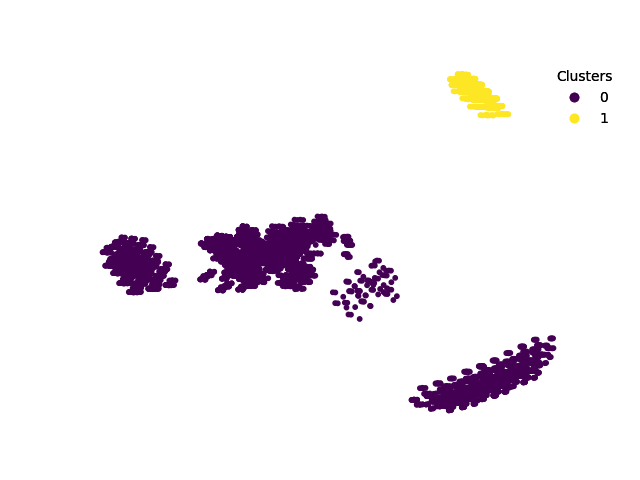
\includegraphics[width=0.8\textwidth]{figures/visualizations/pca_n_components=3,kernel=rbf,gamma=0.1,n_clusters=2,max_iterations=100,tolerance=0.001,random_state=4.png}
    \caption{Clustering visualization for the mushroom dataset using kernel PCA and global k-means clustering.}
    \label{fig:mushroom_clustering}
\end{figure}

The best visualization of the clustering for the vowel dataset demonstrates clear and distinct clusters using PCA reduction combined with global k-means clustering and PCA visualization. This visualization, achieved with the parameters \texttt{PCA\_n\_components=2}, \texttt{n\_clusters=11}, \texttt{max\_iterations=100}, \texttt{tolerance=0.001}, and \texttt{random\_state=4}, effectively separates the dataset's 11 classes in the PCA-transformed 2D space. The clusters are well-separated, reflecting the dataset's inherent class separability despite its challenging distribution. However, while there is no overlap between clusters, some members of the same cluster appear in different corners of the plot, highlighting a limitation in achieving tight cohesion within clusters.

This approach works well for the vowel dataset because its balanced class distribution and absence of missing values align with PCA’s strength in dimensionality reduction and global k-means’ ability to partition data effectively based on variance. Still, the clustering task remains inherently challenging due to the high number of clusters (11) relative to the dataset size, which makes fully cohesive clusters difficult to achieve.

\begin{figure}[h!]
    \centering
    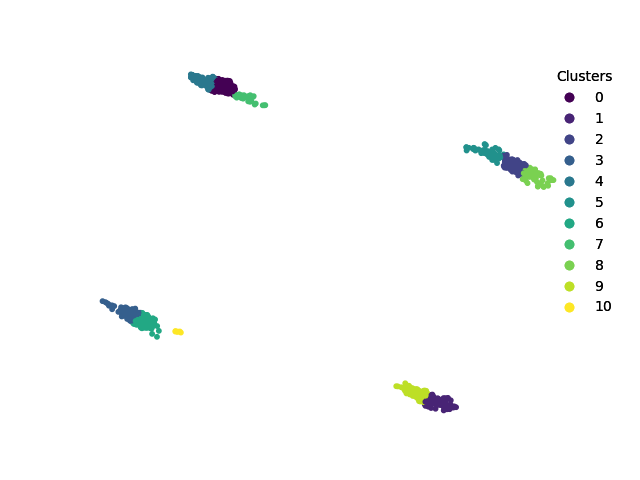
\includegraphics[width=0.8\textwidth]{figures/visualizations/pca_n_components=2,n_clusters=11,max_iterations=100,tolerance=0.001,random_state=4.png}
    \caption{Clustering visualization for the vowel dataset using PCA and global k-means clustering.}
    \label{fig:vowel_clustering}
\end{figure}

UMAP likely performed poorly because it is sensitive to the choice of hyperparameters such as the number of neighbors and the minimum distance, which may not have been well-tuned for the mushroom and vowel datasets' specific structures. Additionally, UMAP focuses on preserving local relationships, which might not align well with the global separability required for effective clustering in these datasets.
